\documentclass{standalone}

\usepackage{tikz,pgf} %and any other packages or tikzlibraries your picture needs

\begin{document}

%%%%%%%%%%%%%%%%%%%%%%%%%%%%%%%%%%%%%%%%%%%%%%%%%%%%%%%%%%%%%%%%%%%%%%%%%%%%%%%%
%COPY HERE
%%%%%%%%%%%%%%%%%%%%%%%%%%%%%%%%%%%%%%%%%%%%%%%%%%%%%%%%%%%%%%%%%%%%%%%%%%%%%%%%


\tikzset{every picture/.style={line width=0.75pt}} %set default line width to 0.75pt

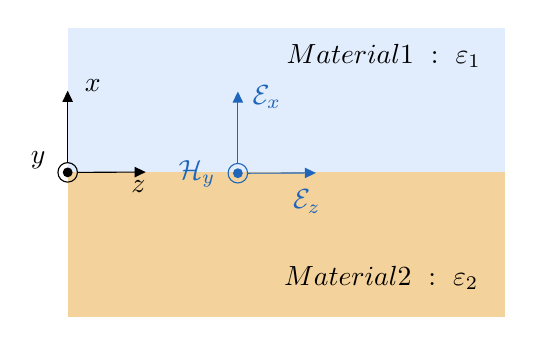
\begin{tikzpicture}[x=0.75pt,y=0.75pt,yscale=-1,xscale=1]
%uncomment if require: \path (0,300); %set diagram left start at 0, and has height of 300

%Shape: Rectangle [id:dp6791714378906519]
\draw  [draw opacity=0][fill={rgb, 255:red, 244; green, 210; blue, 155 }  ,fill opacity=1 ] (164.2,161.55) -- (375,161.55) -- (375,231) -- (164.2,231) -- cycle ;
%Shape: Rectangle [id:dp6526245353151652]
\draw  [draw opacity=0][fill={rgb, 255:red, 225; green, 237; blue, 252 }  ,fill opacity=1 ] (164.2,92.1) -- (375,92.1) -- (375,161.55) -- (164.2,161.55) -- cycle ;

%Shape: Circle [id:dp5883505451182489]
\draw   (159.5,161.55) .. controls (159.5,158.95) and (161.6,156.85) .. (164.2,156.85) .. controls (166.8,156.85) and (168.9,158.95) .. (168.9,161.55) .. controls (168.9,164.15) and (166.8,166.25) .. (164.2,166.25) .. controls (161.6,166.25) and (159.5,164.15) .. (159.5,161.55) -- cycle ;
%Shape: Circle [id:dp21670819657818385]
\draw  [fill={rgb, 255:red, 0; green, 0; blue, 0 }  ,fill opacity=1 ] (162.13,161.55) .. controls (162.13,160.4) and (163.05,159.48) .. (164.2,159.48) .. controls (165.35,159.48) and (166.28,160.4) .. (166.28,161.55) .. controls (166.28,162.7) and (165.35,163.63) .. (164.2,163.63) .. controls (163.05,163.63) and (162.13,162.7) .. (162.13,161.55) -- cycle ;
%Straight Lines [id:da6839540074358363]
\draw    (168.9,161.55) -- (198.8,161.41) ;
\draw [shift={(201.8,161.4)}, rotate = 539.74] [fill={rgb, 255:red, 0; green, 0; blue, 0 }  ][line width=0.08]  [draw opacity=0] (5.36,-2.57) -- (0,0) -- (5.36,2.57) -- cycle    ;
%Straight Lines [id:da13444611152032793]
\draw    (164.2,156.85) -- (164.2,125.2) ;
\draw [shift={(164.2,122.2)}, rotate = 450] [fill={rgb, 255:red, 0; green, 0; blue, 0 }  ][line width=0.08]  [draw opacity=0] (5.36,-2.57) -- (0,0) -- (5.36,2.57) -- cycle    ;
%Shape: Circle [id:dp3939191475485877]
\draw  [color={rgb, 255:red, 31; green, 102; blue, 186 }  ,draw opacity=1 ] (241.5,161.95) .. controls (241.5,159.35) and (243.6,157.25) .. (246.2,157.25) .. controls (248.8,157.25) and (250.9,159.35) .. (250.9,161.95) .. controls (250.9,164.55) and (248.8,166.65) .. (246.2,166.65) .. controls (243.6,166.65) and (241.5,164.55) .. (241.5,161.95) -- cycle ;
%Shape: Circle [id:dp19230827471432965]
\draw  [color={rgb, 255:red, 31; green, 102; blue, 186 }  ,draw opacity=1 ][fill={rgb, 255:red, 31; green, 102; blue, 186 }  ,fill opacity=1 ] (244.13,161.95) .. controls (244.13,160.8) and (245.05,159.88) .. (246.2,159.88) .. controls (247.35,159.88) and (248.28,160.8) .. (248.28,161.95) .. controls (248.28,163.1) and (247.35,164.03) .. (246.2,164.03) .. controls (245.05,164.03) and (244.13,163.1) .. (244.13,161.95) -- cycle ;
%Straight Lines [id:da93825049971561]
\draw [color={rgb, 255:red, 31; green, 102; blue, 186 }  ,draw opacity=1 ][fill={rgb, 255:red, 31; green, 102; blue, 186 }  ,fill opacity=1 ]   (250.9,161.95) -- (280.8,161.81) ;
\draw [shift={(283.8,161.8)}, rotate = 539.74] [fill={rgb, 255:red, 31; green, 102; blue, 186 }  ,fill opacity=1 ][line width=0.08]  [draw opacity=0] (5.36,-2.57) -- (0,0) -- (5.36,2.57) -- cycle    ;
%Straight Lines [id:da27961093495610734]
\draw [color={rgb, 255:red, 31; green, 102; blue, 186 }  ,draw opacity=1 ][fill={rgb, 255:red, 31; green, 102; blue, 186 }  ,fill opacity=1 ]   (246.2,157.25) -- (246.2,125.6) ;
\draw [shift={(246.2,122.6)}, rotate = 450] [fill={rgb, 255:red, 31; green, 102; blue, 186 }  ,fill opacity=1 ][line width=0.08]  [draw opacity=0] (5.36,-2.57) -- (0,0) -- (5.36,2.57) -- cycle    ;


% Text Node
\draw (267.2,205.4) node [anchor=north west][inner sep=0.75pt]    {$Material2\ :\ \varepsilon _{2}$};
% Text Node
\draw (268.4,98.6) node [anchor=north west][inner sep=0.75pt]    {$Material1\ :\ \varepsilon _{1}$};
% Text Node
\draw (171.2,115.6) node [anchor=north west][inner sep=0.75pt]    {$x$};
% Text Node
\draw (145.2,150.4) node [anchor=north west][inner sep=0.75pt]    {$y$};
% Text Node
\draw (193.6,164.4) node [anchor=north west][inner sep=0.75pt]    {$z$};
% Text Node
\draw (252,118.4) node [anchor=north west][inner sep=0.75pt]    {$\textcolor[rgb]{0.12,0.4,0.73}{\mathcal{E}_{x}}$};
% Text Node
\draw (271.6,168.8) node [anchor=north west][inner sep=0.75pt]    {$\textcolor[rgb]{0.12,0.4,0.73}{\mathcal{E}_{z}}$};
% Text Node
\draw (216.4,154.4) node [anchor=north west][inner sep=0.75pt]    {$\textcolor[rgb]{0.12,0.4,0.73}{\mathcal{H}_{y}}$};


\end{tikzpicture}



%%%%%%%%%%%%%%%%%%%%%%%%%%%%%%%%%%%%%%%%%%%%%%%%%%%%%%%%%%%%%%%%%%%%%%%%%%%%%%%%
%COPY HERE
%%%%%%%%%%%%%%%%%%%%%%%%%%%%%%%%%%%%%%%%%%%%%%%%%%%%%%%%%%%%%%%%%%%%%%%%%%%%%%%%

\end{document}
